\documentclass[14pt]{extarticle}
\usepackage{fontspec}
\usepackage{polyglossia}
\usepackage{amsmath}
\usepackage{amssymb}
\usepackage{xcolor}
\usepackage{fancyhdr}
\usepackage{graphicx}
\usepackage{listings}
\usepackage[most]{tcolorbox}
% \usepackage{setspace}
\usepackage{pifont}
\usepackage{enumitem}
\usepackage{titlesec}
\usepackage[bottom]{footmisc}
\usepackage{titling}
\usepackage{minted}
\usepackage{etoolbox}
\usepackage{array}
\usepackage{extsizes}
\usepackage{float}
\usepackage{booktabs}
\usepackage{hyperref}
\usepackage[onehalfspacing]{setspace}
\usepackage[a4paper, top=2.7cm, bottom=2.7cm, left=2.5cm, right=2.5cm, headheight=1.5cm, headsep=0.5cm]{geometry}
\usepackage{tikz}

\usetikzlibrary{automata, positioning, arrows.meta, arrows}

\newfontfamily\emoji{Segoe UI Emoji}

\pagestyle{fancy}

\setmainlanguage[numerals=western]{arabic}
\setotherlanguage{english}
% \newfontfamily\arabicfont[Script=Arabic]{Amiri}
\newfontfamily\arabicfont[Script=Arabic]{Calibri}
\newfontfamily\arabicfonttt[Script=Arabic]{Courier New}

\lstset{
  language=[Sharp]C,
  numbers=left,
  stepnumber=1,
  numbersep=8pt,
  frame=single,
  basicstyle=\ttfamily\small,
  keywordstyle=\color{blue},
  stringstyle=\color{red},
  commentstyle=\color{green!50!black}
}

\newif\ifdetailed
\ifdefined\setdetailed
  \setdetailed
\fi

\newif\ifwithsols
\ifdefined\setwithsols
  \setwithsols
\fi

% unified tcolorboxes for articles
\tcbset{colback=white, colframe=black, fonttitle=\bfseries, boxrule=0.8pt}
\newtcolorbox{boxDef}[1][]{colback=blue!5!white,colframe=blue!75!black,
  title={{\emoji📘} تعريف\ifx\\#1\\\else ~#1\fi :}}
\newtcolorbox{boxExercise}[1][]{colback=cyan!5!white,colframe=cyan!70!black,
  title={{\emoji🧩} تمرين\ifx\\#1\\\else ~#1\fi :}}
\newtcolorbox{boxExample}[1][]{colback=yellow!5!white,colframe=orange!90!black,
  title={{\emoji📝} مثال\ifx\\#1\\\else ~#1\fi :}}
\newtcolorbox{boxNote}[1][]{colback=gray!10!white,colframe=black,
  title={{\emoji✨} ملاحظة\ifx\\#1\\\else ~#1\fi :}}
\newtcolorbox{boxAttention}[1][]{colback=magenta!10!white,colframe=magenta!80!black,
  title={{\emoji🔔} تنبيه\ifx\\#1\\\else ~#1\fi :}}
\newtcolorbox{boxWarning}[1][]{colback=red!5!white,colframe=red!75!black,
  title={{\emoji⚡} ملاحظة هامة\ifx\\#1\\\else ~#1\fi :}}
\newtcolorbox{boxSolution}[1][]{colback=green!5!white,colframe=green!60!black,
  title={{\emoji✅} حل\ifx\\#1\\\else ~#1\fi :}}
\newtcolorbox{boxSymbol}[1][]{colback=purple!5!white,colframe=purple!70!black,
  title={{\emoji🔣} رمز\ifx\\#1\\\else ~#1\fi :}}
\newtcolorbox{boxHint}[1][]{colback=teal!5!white,colframe=teal!60!black,
  title={{\emoji💡} تلميح\ifx\\#1\\\else ~#1\fi :}}


\tcbset{simplecode/.style={ colback=gray!5, colframe=black!50, boxrule=0.4pt, arc=2pt, left=4pt,right=4pt,top=4pt,bottom=4pt}}
\newenvironment{boxCode}{\begin{tcolorbox}[simplecode]}{\end{tcolorbox}}

\newcolumntype{C}[1]{>{\centering\arraybackslash}p{#1}}

% redefine spaces after titles
\makeatletter
\renewcommand{\@maketitle}{%
  \begin{center}
    {\huge \bfseries \@title \par}%
    \vskip 0.2em % space between title and author
    {\large \@author \par}%
    % \vskip 0.2em % space between author and date
    % {\normalsize \@date \par}%
  \end{center}
}
\makeatother

\fancyhf{} % clear default
\fancypagestyle{plain}{
  \fancyhf{}
  \fancyhead[L]{مدرسة التسامح الشاملة}
  % \fancyhead[L]{
\includegraphics[height=1cm]{../../../images/logoTasamoh.png}}
  \fancyhead[R]{الأستاذ محمود اغبارية}
  \fancyfoot[C]{\thepage}
}

\fancyhead[L]{مدرسة التسامح الشاملة}
\fancyhead[R]{الأستاذ محمود اغبارية}
\fancyfoot[C]{\thepage}
% \date{\today}

\setcounter{tocdepth}{3} % only section subsection and subsubsection in TOC

\newcommand{\importpdfpage}[2]{%
    \thispagestyle{empty}
    \newgeometry{left=0cm,right=0cm,top=0cm,bottom=0cm}
    \includegraphics[page=#2,width=0.95\paperwidth,height=0.95\paperheight,keepaspectratio]{#1}
    \restoregeometry
}

\newcommand{\insertFullImg}[1]{%
    \noindent
    \makebox[\textwidth][c]{
        \includegraphics[width=0.9\paperwidth,keepaspectratio]{#1}%
    }%
}%

% ----------------------


% \begin{document}

% \maketitle

% % \clearpage  % start TOC on a new page
% % \renewcommand{\contentsname}{جدول المحتويات}
% % \tableofcontents
% % \clearpage

% \part*{part 1} % the * prevents numbering
% \section*{مقدمة}
% \subsection*{مثال رياضي}
% \subsubsection*{مثال فرعي}
% \paragraph*{ paragraph 1}
% \subparagraph*{sub paragraph 1}

% \ifdetailed
% \begin{english}
% \begin{minted}{csharp}
% // C# Example
% \end{minted}
% \end{english}
% \fi

% OLD WAY
% \ifdetailed
% \begin{english}
% \begin{lstlisting}
% // C# Example
% \end{lstlisting}
% \end{english}
% \fi

% % 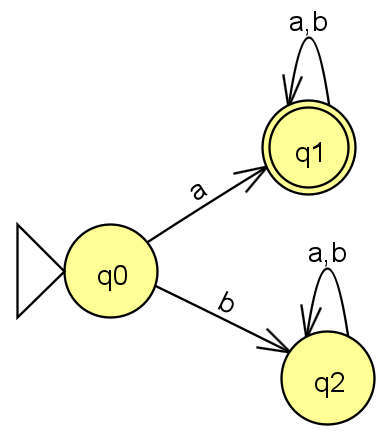
\includegraphics[width=0.2\textwidth]{../../../images/DFAs/ex1_q1.png}



% \vspace{3cm}
% \begin{flushleft}
% أرجو لكم وقتًا ممتعًا.

% الأستاذ محمود اغبارية.
% \end{flushleft}


% \end{document}


\ifwithsols
\title{حل وظيفة 16 - الحلقات المتداخلة}
\else
\title{وظيفة 16 - الحلقات المتداخلة}
\fi

\begin{document}

\maketitle
\thispagestyle{fancy}

\begin{enumerate}[itemsep=2em]
    \item
    اكتب عملية خارجية \textenglish{PrintAllPairs} تتلقى مصفوفة أعداد صحيحة وتطبع جميع الأزواج الممكنة من عناصر المصفوفة.\\
    \textbf{ملاحظة:} كل زوج يطبع مرة واحدة فقط (لا نطبع الزوج المعكوس).\\
    \textbf{مثال:} في المصفوفة \textenglish{\{5, 10, 15, 20\}}، النتيجة:
    \begin{english}
        \begin{boxCode}
        \begin{verbatim}
(5, 10)
(5, 15)
(5, 20)
(10, 15)
(10, 20)
(15, 20)
\end{verbatim}
\end{boxCode}
\end{english}

    \begin{boxHint}
        اكتب حلقتين متداخلتين، واطبع $(arr[i], arr[j])$ في الحلقة الداخلية. تأكد أن الحلقة الداخلية تبدأ من \textenglish{j = i + 1}.
    \end{boxHint}
    \ifwithsols
    \begin{boxSolution}
    \begin{english}
    \begin{minted}{csharp}
public static void PrintAllPairs(int[] arr)
{
    for (int i = 0; i < arr.Length; i++)
    {
        for (int j = i + 1; j < arr.Length; j++)
        {
            Console.WriteLine($"({arr[i]}, {arr[j]})");
        }
    }
}
    \end{minted}
    \end{english}
    \textbf{الشرح:} نفس المنطق من السؤال السابق - الحلقة الداخلية تبدأ من \textenglish{j = i + 1} لضمان عدم طباعة العنصر مع نفسه وعدم طباعة كل زوج مرة واحدة فقط.
    \end{boxSolution}
    \clearpage
    \fi

    \item
    اكتب عملية خارجية \textenglish{PrintPairsWithSum} تتلقى مصفوفة أعداد صحيحة وعددًا صحيحًا، وتطبع جميع أزواج الأرقام في المصفوفة التي مجموعها يساوي العدد المعطى.\\
    \textbf{مثال:} في المصفوفة \textenglish{\{2, 4, 3, 5, 7, 8, 1\}} مع \textenglish{target = 9}، النتيجة:
    \begin{english}
        \begin{boxCode}
    \begin{verbatim}
2 + 7 = 9
4 + 5 = 9
8 + 1 = 9
    \end{verbatim}
\end{boxCode}
    \end{english}
    \ifwithsols
    \begin{boxSolution}
    \begin{english}
    \begin{minted}{csharp}
public static void PrintPairsWithSum(int[] arr, int target)
{
    for (int i = 0; i < arr.Length; i++)
    {
        for (int j = i + 1; j < arr.Length; j++)
        {
            if (arr[i] + arr[j] == target)
            {
                Console.WriteLine($"{arr[i]} + {arr[j]} = {target}");
            }
        }
    }
}
    \end{minted}
    \end{english}
    \textbf{الشرح:} الحلقة الداخلية تبدأ من \textenglish{j = i + 1} (وليس من 0) لتجنب مقارنة العنصر مع نفسه ولتجنب طباعة نفس الزوج مرتين.
    \end{boxSolution}
    \fi

    \clearpage
    \item \textbf{سؤال اختياري} \\
    اكتب عملية خارجية \textenglish{CountGreaterAfter} تتلقى مصفوفة أعداد صحيحة وتعيد مصفوفة جديدة بنفس الطول. كل عنصر في المصفوفة الجديدة يحتوي على عدد العناصر الأكبر منه التي تظهر بعده في المصفوفة الأصلية.\\
    \textbf{مثال 1:} في المصفوفة \textenglish{\{5, 3, 7, 2, 8\}}، النتيجة \textenglish{\{2, 2, 1, 1, 0\}} لأنّ:
    \begin{itemize}[itemsep=1pt]
        \item العنصر 5: بعده يوجد عددان أكبر منه (7 و8) $\rightarrow$ 2
        \item العنصر 3: بعده يوجد عددان أكبر منه (7 و8) $\rightarrow$ 2
        \item العنصر 7: بعده يوجد عدد واحد أكبر منه (8) $\rightarrow$ 1
        \item العنصر 2: بعده يوجد عدد واحد أكبر منه (8) $\rightarrow$ 1
        \item العنصر 8: لا يوجد شيء بعده $\rightarrow$ 0
    \end{itemize}
    \textbf{مثال 2:} في المصفوفة \textenglish{\{10, 8, 6, 4, 2\}}، النتيجة \textenglish{\{0, 0, 0, 0, 0\}} (مصفوفة تنازلية).\\
    \textbf{مثال 3:} في المصفوفة \textenglish{\{1, 2, 3, 4, 5\}}، النتيجة \textenglish{\{4, 3, 2, 1, 0\}} (مصفوفة تصاعدية).
    \ifwithsols
    \begin{boxSolution}
    \begin{english}
    \begin{minted}{csharp}
public static int[] CountGreaterAfter(int[] arr)
{
    int[] result = new int[arr.Length];

    for (int i = 0; i < arr.Length; i++)
    {
        int count = 0;

        // نمر على جميع العناصر بعد الموقع i
        for (int j = i + 1; j < arr.Length; j++)
        {
            if (arr[j] > arr[i])
            {
                count++;
            }
        }

        result[i] = count;
    }

    return result;
}
    \end{minted}
    \end{english}
    \textbf{الشرح:}
    \begin{itemize}[itemsep=1pt]
        \item ننشئ مصفوفة جديدة \textenglish{result} بنفس طول المصفوفة الأصلية
        \item الحلقة الخارجية تمر على كل عنصر في الموقع \textenglish{i}
        \item لكل عنصر، ننشئ متغير عداد \textenglish{count = 0}
        \item الحلقة الداخلية تبدأ من \textenglish{j = i + 1} (العناصر بعد الموقع \textenglish{i})
        \item نفحص: هل \textenglish{arr[j] > arr[i]}؟ إذا نعم، نزيد العداد
        \item نخزن قيمة العداد في \textenglish{result[i]}
    \end{itemize}
    \end{boxSolution}
    \fi

\end{enumerate}

\vspace{1cm}
\begin{flushleft}
أرجو لكم عملاً ممتعاً!

الأستاذ محمود اغبارية.
\end{flushleft}

\end{document}